\documentclass[11pt]{report}
\usepackage{tikz}
\usetikzlibrary{fit,positioning}
\begin{document}
\begin{figure}
\centering
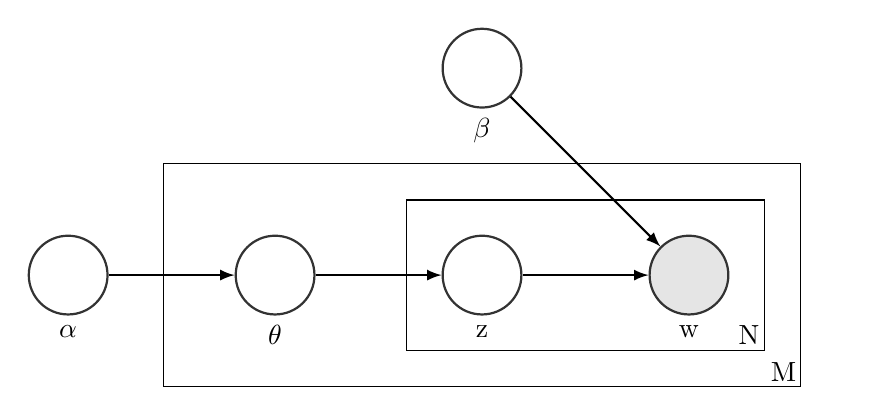
\begin{tikzpicture}
%\tikzstyle{main}=[circle, minimum size = 10mm, thick, draw =black!80, node distance = 16mm]
%\tikzstyle{connect}=[-latex, thick]
%\tikzstyle{box}=[rectangle, draw=black!100]
%  \node[main, fill = white!100] (alpha) [label=below:$\alpha$] { };
%  \node[main] (theta) [right=of alpha,label=below:$\theta$] { };
%  \node[main] (z) [right=of theta,label=below:z] {};
%  \node[main] (beta) [above=of z,label=below:$\beta$] { };
%  \node[main, fill = black!10] (w) [right=of z,label=below:w] { };
%  \path (alpha) edge [connect] (theta)
%        (theta) edge [connect] (z)
%		(z) edge [connect] (w)
%		(beta) edge [connect] (w);
%  \node[rectangle, inner sep=0mm, fit= (z) (w),label=below right:N, xshift=13mm] {};
%  \node[rectangle, inner sep=4.4mm,draw=black!100, fit= (z) (w)] {};
%  \node[rectangle, inner sep=4.6mm, fit= (z) (w),label=below right:M, xshift=12.5mm] {};
%  \node[rectangle, inner sep=9mm, draw=black!100, fit = (theta) (z) (w)] {};
\tikzstyle{main}=[circle, minimum size = 10mm, thick, draw =black!80, node distance = 16mm]
\tikzstyle{connect}=[-latex, thick]
\tikzstyle{box}=[rectangle, draw=black!100]
  \node[main, fill = white!100] (alpha) [label=below:$\alpha$] { };
  \node[main] (theta) [right=of alpha,label=below:$\theta$] { };
  \node[main] (z) [right=of theta,label=below:z] {};
  \node[main] (beta) [above=of z,label=below:$\beta$] { };
  \node[main, fill = black!10] (w) [right=of z,label=below:w] { };
  \path (alpha) edge [connect] (theta)
        (theta) edge [connect] (z)
		(z) edge [connect] (w)
		(beta) edge [connect] (w);
  \node[rectangle, inner sep=0mm, fit= (z) (w),label=below right:N, xshift=13mm] {};
  \node[rectangle, inner sep=4.4mm,draw=black!100, fit= (z) (w)] {};
  \node[rectangle, inner sep=4.6mm, fit= (z) (w),label=below right:M, xshift=12.5mm] {};
  \node[rectangle, inner sep=9mm, draw=black!100, fit = (theta) (z) (w)] {};
\end{tikzpicture}
\end{figure}

\begin{equation}
weight_k = w_k  \sim Dir(\vec{\alpha_0})\
\end{equation}

\begin{equation}
phaseweight_k = \bar{w}_k  \sim Dir(\vec{w}^T\vec{\alpha_1} )\
\end{equation}

\begin{equation}
locs_k = c_k  \sim N(\vec{0}, \vec{I})
\end{equation}

\begin{equation}
scale_d = s_d  \sim U(\gamma / 2, 3 \gamma / 2)
\end{equation}


\begin{equation}
obs_i = y_i = N(\vec{\bar{w}}^T \vec{c}, \Sigma)
\end{equation}

\end{document}
\end{document}
